\section{Data Warehouse Modeling: Data Cube and OLAP}

% TODO: Example ERM for sales

\begin{frame}{Data Cubes}
	\begin{itemize}
		\item Data warehouse is based on a \textbf{\color{airforceblue}multidimensional data model}
		\item It views data in the form of a \textbf{data cube}.
		\item A {\color{faugray}\textbf{data cube}} contains \textbf{two} different kinds of data:
		      \begin{itemize}
			      \item \textbf{Dimensions:} Information that can be used to group the data.
			            \begin{itemize}
				            \item A dimension often comes with different levels of granularity.
				            \item Example: Time (Granularity levels: day, month, quarter, year).
			            \end{itemize}
			      \item \textbf{Facts}: Information that can be aggregated.
			            \begin{itemize}
				            \item Example: Price.
			            \end{itemize}
		      \end{itemize}
	\end{itemize}
\end{frame}

\begin{frame}{Example: 3-D Data Cube}
	\begin{center}
		\scalebox{0.875}{
			\begin{tikzpicture}[scale=1]
				% Important: 
				% If the coordinates are x, y, z then:
				% x = 0 is the left side, x = 4 is the right side
				% y = 0 is the bottom side, y = 4 is the top side
				% z = 0 is the back side, z = 4 is the front side
				% 
				% To get the left bottom corner of the cube, use (0,0,4):
				% \fill[black] (0,0,4) circle (1.5pt);
				\useasboundingbox (-2.5,-1.8,4) rectangle (12,4,-1);

				% 1. STEP - Talking points:
				% - Imagine a three-dimensional coordinate system

				\only<1>{
					\node[text width=5cm, anchor=west] at (7.75,2.5,4) {
						\begin{block}{Imagine:}
							\begin{itemize}
								\item 3-D coordinate system
							\end{itemize}
						\end{block}
					};
				}

				% Only axis
				\only<1-3>{
					\draw[->] (0,0,4) -- (0,5,4);
					\draw[->] (0,0,4) -- (5,0,4);
					\draw[->] (0,0,4) -- (0,0,-1);
				}

				% Axis labels
				\only<1-4>{
					\node[anchor=south,rotate=90] at (-0.25,2.5,4) {\texttt{Time}};
					\node[anchor=north] at (2.5,-0.25,4) {\texttt{Region}};
					\node[anchor=south,rotate=45] at (-0.125,0.125,1.5) {\texttt{Product}};
				}

				% 2. STEP - Talking points:
				% - Individual data points can be located anywhere in this coordinate system

				\only<2>{
					\node[text width=5cm, anchor=west] at (7.75,2.5,4) {
						\begin{block}{Dimensional Values:}
							\begin{itemize}
								\item Used to locate data points
								\item Example: Erlangen/Bavaria/Germany,\\ 01/05/2Q/2023,\\ Series 8/Washer
							\end{itemize}
						\end{block}
						\begin{block}{Facts:}
							\begin{itemize}
								\item Used to describe data points
								\item Example: 430€
							\end{itemize}
						\end{block}
					};
				}

				% Add data points with labels 
				\only<2>{
					\fill[black] (1.3,0.3,3.9) circle (1.5pt) node[above right] {\tiny{(Erlangen/Bavaria/Germany, 01/05/2Q/2023, Series 8/Washer) - (430€)}};
					\fill[black] (3.9,1.4,0.3) circle (1.5pt) node[above left] {\tiny{(Rome/Lazio/Italy, 23/06/2Q/2024, ePhone 16/Phone) - (1250€)}};
				}

				\only<3>{
					\node[text width=5cm, anchor=west] at (7.75,2.5,4) {
						\begin{block}{A Real Data Cube:}
							\begin{itemize}
								\item Contains a lot of data points
								\item Many more than shown ...
							\end{itemize}
						\end{block}
					};
				}

				% Also add a lot more without labels 
				\only<3-6>{
					\fill[gray] (0.4,0.3,1.3) circle (1.5pt);
					\fill[gray] (0.5,1.9,1.8) circle (1.5pt);
					\fill[gray] (1.2,0.5,2.1) circle (1.5pt);
					\fill[gray] (1.5,0.8,2.4) circle (1.5pt);
					\fill[gray] (1.8,0.2,2.7) circle (1.5pt);
					\fill[gray] (2.1,1.6,1.0) circle (1.5pt);
					\fill[gray] (2.4,0.9,3.3) circle (1.5pt);
					\fill[gray] (2.7,3.2,3.6) circle (1.5pt);
					%\fill[gray] (1.0,1.5,3.9) circle (1.5pt);
					\fill[gray] (3.3,2.8,3.2) circle (1.5pt);
					\fill[gray] (3.6,2.1,3.5) circle (1.5pt);
					\fill[gray] (3.6,2.1,3.5) circle (1.5pt);
					\fill[gray] (3.9,1.4,4) circle (1.5pt);
					% ...
				}

				% Repetition of the previously labeled data points (now without labels)
				\only<3-6>{
					\fill[black] (1.3,0.3,3.9) circle (1.5pt);
					\fill[black] (3.9,1.4,0.3) circle (1.5pt);
				}

				% 3. STEP - Talking points:
				% - All these data points can be grouped into a cube
				% - The facts (e.g. prices) of all the data points in the cube can be aggregated

				\only<4>{
					\node[text width=5cm, anchor=west] at (7.75,2.5,4) {
						\begin{block}{The Data Cube:}
							\begin{itemize}
								\item Encapsulates all data points
								\item Can be used to aggregate all facts
							\end{itemize}
						\end{block}
					};
				}

				% Repetition of the axis (taking the cube into account)
				\only<4>{
					\draw[->] (0,0,4) -- (0,5,4);
					\draw[->] (0,0,4) -- (5,0,4);
					\draw[->, dashed] (0,0,4) -- (0,0,-1);
				}

				% Cube
				\only<4>{
					\foreach \x in{0,4,...,4}
						{   \draw (0,\x ,4) -- (4,\x ,4);
							\draw (\x ,0,4) -- (\x ,4,4);
							\draw (4,\x ,4) -- (4,\x ,0);
							\draw (\x ,4,4) -- (\x ,4,0);
							\draw (4,0,\x ) -- (4,4,\x );
							\draw (0,4,\x ) -- (4,4,\x );
						}
				}

				% 4. STEP - Talking points:
				% - The cube can be sliced into smaller cubes for more detailed analysis
				% - There aggregation on the facts of a smaller cube can be performed

				\only<5>{
					\node[text width=5cm, anchor=west] at (7.75,2.5,4) {
						\begin{block}{A Cube of Cubes:}
							\begin{itemize}
								\item The cube can be sliced into smaller cubes
							\end{itemize}
						\end{block}
						\begin{block}{The Smaller Cubes:}
							\begin{itemize}
								\item Can be analyzed separately
								\item Are in the highest granularity of each dimension
							\end{itemize}
						\end{block}
					};
				}

				% Highest granularity cube
				\only<5>{
					\foreach \x in{0,...,4}
						{   \draw (0,\x ,4) -- (4,\x ,4);
							\draw (\x ,0,4) -- (\x ,4,4);
							\draw (4,\x ,4) -- (4,\x ,0);
							\draw (\x ,4,4) -- (\x ,4,0);
							\draw (4,0,\x ) -- (4,4,\x );
							\draw (0,4,\x ) -- (4,4,\x );
						}
				}

				% Axis categories (highest granularity)
				\only<5>{
					% Time axis
					\node[anchor=east] at (-0.25,0.5,4) {\texttt{2023}};
					\node[anchor=east] at (-0.25,1.5,4) {\texttt{2024}};
					\node[anchor=east] at (-0.25,2.5,4) {\texttt{2025}};
					\node[anchor=east] at (-0.25,3.5,4) {\texttt{2026}};

					% Region axis 
					\node[anchor=east,rotate=90] at (0.5, -0.25, 4) {\texttt{France}};
					\node[anchor=east,rotate=90] at (1.5, -0.25, 4) {\texttt{Germany}};
					\node[anchor=east,rotate=90] at (2.5, -0.25, 4) {\texttt{Spain}};
					\node[anchor=east,rotate=90] at (3.5, -0.25, 4) {\texttt{Italy}};

					% Product axis
					\node[anchor=west,rotate=315] at (4.125, -0.125, 3.5) {\texttt{Washer}};
					\node[anchor=west,rotate=315] at (4.125, -0.125, 2.5) {\texttt{Fridge}};
					\node[anchor=west,rotate=315] at (4.125, -0.125, 1.5) {\texttt{TV}};
					\node[anchor=west,rotate=315] at (4.125, -0.125, 0.5) {\texttt{Phone}};
				}

				% 5. STEP - Talking points:
				% - The cube can be even be sliced into smaller cubes for more detailed analysis
				% - In this example we only go to the next granularity level in the time dimension
				% - The other dimensions also have finer granularity levels
				% - More on this on a later slide

				\only<6>{
					\node[text width=5cm, anchor=west] at (7.75,2.5,4) {
						\begin{block}{Even Smaller Cubes:}
							\begin{itemize}
								\item Often the cubes can be sliced into even smaller cubes
								\item By going to the next finer granularity level in at least one dimension
							\end{itemize}
						\end{block}
					};
				}

				% Next granularity cube
				\only<6>{
					\foreach \y in{0,0.25,...,4}
						{
							\foreach \xz in{0,1,...,4}
								{   \draw (0,\y ,4) -- (4,\y ,4);
									\draw (\xz ,0,4) -- (\xz ,4,4);
									\draw (4,\y ,4) -- (4,\y ,0);
									\draw (\xz ,4,4) -- (\xz ,4,0);
									\draw (4,0,\xz ) -- (4,4,\xz );
									\draw (0,4,\xz ) -- (4,4,\xz );
								}
						}
				}

				% Axis categories (highest granularity)
				\only<6>{
					% Time axis
					\node[anchor=east] at (-1.25,0.5,4) {\texttt{2023}};
					\node[anchor=east] at (-0.25,0.125,4) {\small{\texttt{Q1}}};
					\node[anchor=east] at (-0.25,0.375,4) {\small{\texttt{Q2}}};
					\node[anchor=east] at (-0.25,0.625,4) {\small{\texttt{Q3}}};
					\node[anchor=east] at (-0.25,0.875,4) {\small{\texttt{Q4}}};
					\node[anchor=east] at (-1.25,1.5,4) {\texttt{2024}};
					\node[anchor=east] at (-0.25,1.125,4) {\small{\texttt{Q1}}};
					\node[anchor=east] at (-0.25,1.375,4) {\small{\texttt{Q2}}};
					\node[anchor=east] at (-0.25,1.625,4) {\small{\texttt{Q3}}};
					\node[anchor=east] at (-0.25,1.875,4) {\small{\texttt{Q4}}};
					\node[anchor=east] at (-1.25,2.5,4) {\texttt{2025}};
					\node[anchor=east] at (-0.25,2.125,4) {\small{\texttt{Q1}}};
					\node[anchor=east] at (-0.25,2.375,4) {\small{\texttt{Q2}}};
					\node[anchor=east] at (-0.25,2.625,4) {\small{\texttt{Q3}}};
					\node[anchor=east] at (-0.25,2.875,4) {\small{\texttt{Q4}}};
					\node[anchor=east] at (-1.25,3.5,4) {\texttt{2026}};
					\node[anchor=east] at (-0.25,3.125,4) {\small{\texttt{Q1}}};
					\node[anchor=east] at (-0.25,3.375,4) {\small{\texttt{Q2}}};
					\node[anchor=east] at (-0.25,3.625,4) {\small{\texttt{Q3}}};
					\node[anchor=east] at (-0.25,3.875,4) {\small{\texttt{Q4}}};

					% Region axis 
					\node[anchor=east,rotate=90] at (0.5, -0.25, 4) {\texttt{France}};
					\node[anchor=east,rotate=90] at (1.5, -0.25, 4) {\texttt{Germany}};
					\node[anchor=east,rotate=90] at (2.5, -0.25, 4) {\texttt{Italy}};
					\node[anchor=east,rotate=90] at (3.5, -0.25, 4) {\texttt{Spain}};

					% Product axis
					\node[anchor=west,rotate=315] at (4.125, -0.125, 3.5) {\texttt{Washer}};
					\node[anchor=west,rotate=315] at (4.125, -0.125, 2.5) {\texttt{Fridge}};
					\node[anchor=west,rotate=315] at (4.125, -0.125, 1.5) {\texttt{TV}};
					\node[anchor=west,rotate=315] at (4.125, -0.125, 0.5) {\texttt{Phone}};
				}


			\end{tikzpicture}
		}
	\end{center}
\end{frame}

\begin{frame}{mE/R Model of a Data Cube}
	\begin{itemize}
		\item A \textbf{mE/R model}\footnote{\fullcite{sapia98}} contains both \textbf{dimensions} and \textbf{facts}.
		\item Very good in representing \textbf{dimensional hierarchies}.
	\end{itemize}

	\vspace*{3mm}

	\begin{center}
		\scalebox{0.85}{
			\begin{tikzpicture}
				% Cube
				\foreach \x in{0,2,...,2}
					{   \draw (0,\x ,2) -- (2,\x ,2);
						\draw (\x ,0,2) -- (\x ,2,2);
						\draw (2,\x ,2) -- (2,\x ,0);
						\draw (\x ,2,2) -- (\x ,2,0);
						\draw (2,0,\x ) -- (2,2,\x );
						\draw (0,2,\x ) -- (2,2,\x );
					}

				% Title
				\node at (1,1.75,2) {\footnotesize{Sales}};

				% Titel line
				\draw (0,1.5,2) -- (2,1.5,2);

				% Fact(s)
				\node[darkgray] at (1,1.25,2) {\footnotesize{Price}};

				% Dimension(s)
				% --- Time ---
				% Nodes
				\node[draw, rectangle, minimum width=1.5cm, minimum height=0.5cm, align=center] (day) at (-2,3,2) {\footnotesize{Day}};
				\node[draw, rectangle, minimum width=1.5cm, minimum height=0.5cm, align=center] (month) at (-4,3,2) {\footnotesize{Month}};
				\node[draw, rectangle, minimum width=1.5cm, minimum height=0.5cm, align=center] (week) at (-4,2.25,2) {\footnotesize{Week}};
				\node[draw, rectangle, minimum width=1.5cm, minimum height=0.5cm, align=center] (quarter) at (-6,3,2) {\footnotesize{Quarter}};
				\node[draw, rectangle, minimum width=1.5cm, minimum height=0.5cm, align=center] (year) at (-8,3,2) {\footnotesize{Year}};
				% Connection Cube -> Day
				\draw (0,1,2) -- (day.east);
				% Connection Day -> Month
				\draw ($(day.west) + (0,0.1,0)$) -- ($(day.west) + (-0.1,0,0)$);
				\draw ($(day.west) + (0,-0.1,0)$) -- ($(day.west) + (-0.1,0,0)$);
				\draw[->] ($(day.west) + (-0.1,0,0)$) -- (month.east);
				% Connection Month -> Quarter
				\draw ($(month.west) + (0,0.1,0)$) -- ($(month.west) + (-0.1,0,0)$);
				\draw ($(month.west) + (0,-0.1,0)$) -- ($(month.west) + (-0.1,0,0)$);
				\draw[->] ($(month.west) + (-0.1,0,0)$) -- (quarter.east);
				% Connection Quarter -> Year
				\draw ($(quarter.west) + (0,0.1,0)$) -- ($(quarter.west) + (-0.1,0,0)$);
				\draw ($(quarter.west) + (0,-0.1,0)$) -- ($(quarter.west) + (-0.1,0,0)$);
				\draw[->] ($(quarter.west) + (-0.1,0,0)$) -- (year.east);
				% Connection Day -> Week
				\draw ($(day.south) + (0.1,0,0)$) -- ($(day.south) + (0,-0.1,0)$);
				\draw ($(day.south) + (-0.1,0,0)$) -- ($(day.south) + (0,-0.1,0)$);
				\draw[->] ($(day.south) + (0,-0.1,0)$) |- (week.east);

				% --- Region ---
				% Nodes
				\node[draw, rectangle, minimum width=1.5cm, minimum height=0.5cm, align=center] (city) at (-2,1,2) {\footnotesize{City}};
				\node[draw, rectangle, minimum width=1.5cm, minimum height=0.5cm, align=center] (region) at (-4,1,2) {\footnotesize{Region}};
				\node[draw, rectangle, minimum width=1.5cm, minimum height=0.5cm, align=center] (country) at (-6,1,2) {\footnotesize{Country}};
				% Connection Cube -> City
				\draw (0,1,2) -- (city.east);
				% Connection City -> Region
				\draw ($(city.west) + (0,0.1,0)$) -- ($(city.west) + (-0.1,0,0)$);
				\draw ($(city.west) + (0,-0.1,0)$) -- ($(city.west) + (-0.1,0,0)$);
				\draw[->] ($(city.west) + (-0.1,0,0)$) -- (region.east);
				% Connection Region -> Country
				\draw ($(region.west) + (0,0.1,0)$) -- ($(region.west) + (-0.1,0,0)$);
				\draw ($(region.west) + (0,-0.1,0)$) -- ($(region.west) + (-0.1,0,0)$);
				\draw[->] ($(region.west) + (-0.1,0,0)$) -- (country.east);


				% --- Product ---
				% Nodes
				\node[draw, rectangle, minimum width=1.5cm, minimum height=0.5cm, align=center] (item) at (-2,-1,2) {\footnotesize{Item}};
				\node[draw, rectangle, minimum width=1.5cm, minimum height=0.5cm, align=center] (category) at (-4,-1,2) {\footnotesize{Category}};
				% Connection Cube -> Item
				\draw (0,1,2) -- (item.east);
				% Connection Item -> Category
				\draw ($(item.west) + (0,0.1,0)$) -- ($(item.west) + (-0.1,0,0)$);
				\draw ($(item.west) + (0,-0.1,0)$) -- ($(item.west) + (-0.1,0,0)$);
				\draw[->] ($(item.west) + (-0.1,0,0)$) -- (category.east);
			\end{tikzpicture}
		}
	\end{center}
\end{frame}

\begin{frame}{Narrowing the Data Cube Down}
	\begin{itemize}
		\item Each data cube can be aggregated.
		\item In this process, it is possible to use only individual dimensions for aggregation:
		      \begin{itemize}
			      \item \textbf{$n$-dimensional base cube.}
			            \begin{itemize}
				            \item Called a base cuboid in data warehousing literature.
			            \end{itemize}
			      \item \textbf{Top most $0$-dimensional cuboid.}
			            \begin{itemize}
				            \item Holds the highest-level of summarization.
				            \item Called the apex cuboid.
			            \end{itemize}
			      \item \textbf{Lattice of cuboids.} (Forms a data cube)
		      \end{itemize}
	\end{itemize}
\end{frame}

\begin{frame}{Cube: A Lattice of Cuboids}
	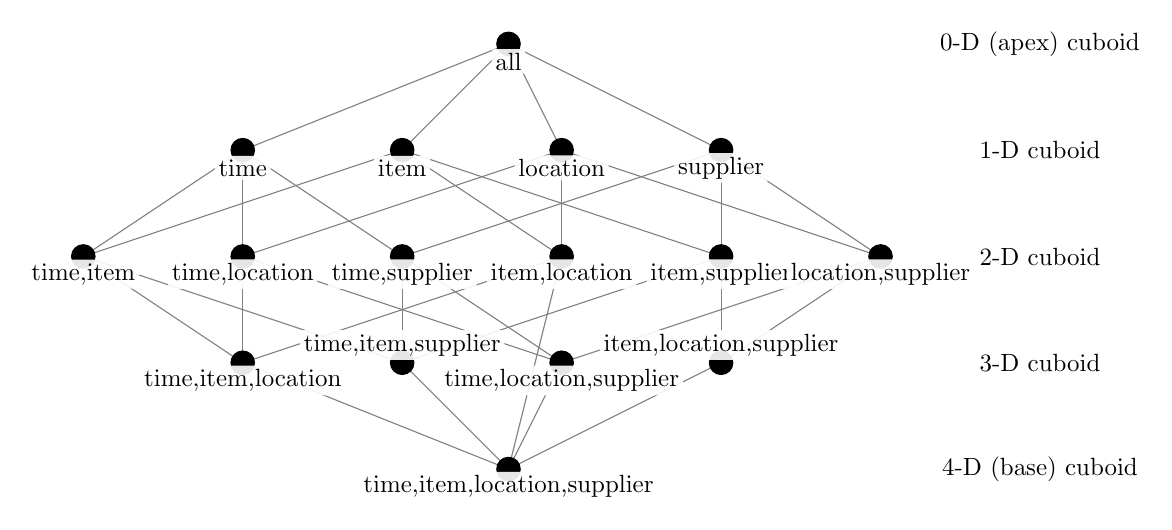
\begin{tikzpicture}[
			scale=0.9,
			every node/.style={transform shape}
		]
		% Connections
		\draw[gray] (3,6) -- (-0.75,4.5);
		\draw[gray] (3,6) -- (1.5,4.5);
		\draw[gray] (3,6) -- (3.75,4.5);
		\draw[gray] (3,6) -- (6,4.5);

		\draw[gray] (-0.75,4.5) -- (-3,3);
		\draw[gray] (-0.75,4.5) -- (-0.75,3);
		\draw[gray] (-0.75,4.5) -- (1.5,3);
		\draw[gray] (1.5,4.5) -- (-3,3);
		\draw[gray] (1.5,4.5) -- (3.75,3);
		\draw[gray] (1.5,4.5) -- (6,3);
		\draw[gray] (3.75,4.5) -- (-0.75,3);
		\draw[gray] (3.75,4.5) -- (3.75,3);
		\draw[gray] (3.75,4.5) -- (8.25,3);
		\draw[gray] (6,4.5) -- (1.5,3);
		\draw[gray] (6,4.5) -- (6,3);
		\draw[gray] (6,4.5) -- (8.25,3);

		\draw[gray] (-3,3) -- (-0.75,1.5);
		\draw[gray] (-3,3) -- (1.5,1.5);
		\draw[gray] (-0.75,3) -- (-0.75,1.5);
		\draw[gray] (-0.75,3) -- (3.75,1.5);
		\draw[gray] (1.5,3) -- (1.5,1.5);
		\draw[gray] (1.5,3) -- (3.75,1.5);
		\draw[gray] (3.75,3) -- (-0.75,1.5);
		\draw[gray] (3.75,3) -- (3,0);
		\draw[gray] (6,3) -- (1.5,1.5);
		\draw[gray] (6,3) -- (6,1.5);
		\draw[gray] (8.25,3) -- (3.75,1.5);
		\draw[gray] (8.25,3) -- (6,1.5);

		\draw[gray] (-0.75,1.5) -- (3,0);
		\draw[gray] (1.5,1.5) -- (3,0);
		\draw[gray] (3.75,1.5) -- (3,0);
		\draw[gray] (6,1.5) -- (3,0);

		% Nodes
		\node[draw, circle, fill=black] at (3,6) {};
		\node[draw, circle, fill=black] at (-0.75,4.5) {};
		\node[draw, circle, fill=black] at (1.5,4.5) {};
		\node[draw, circle, fill=black] at (3.75,4.5) {};
		\node[draw, circle, fill=black] at (6,4.5) {};

		\node[draw, circle, fill=black] at (-3,3) {};
		\node[draw, circle, fill=black] at (-0.75,3) {};
		\node[draw, circle, fill=black] at (1.5,3) {};
		\node[draw, circle, fill=black] at (3.75,3) {};
		\node[draw, circle, fill=black] at (6,3) {};
		\node[draw, circle, fill=black] at (8.25,3) {};

		\node[draw, circle, fill=black] at (-0.75,1.5) {};
		\node[draw, circle, fill=black] at (1.5,1.5) {};
		\node[draw, circle, fill=black] at (3.75,1.5) {};
		\node[draw, circle, fill=black] at (6,1.5) {};

		\node[draw, circle, fill=black] at (3,0) {};

		% Labels
		\node[fill=white, text opacity=1, fill opacity=0.9, inner sep=1.5pt, rounded corners=1pt] at (3,5.75) {all};

		\node[fill=white, text opacity=1, fill opacity=0.9, inner sep=1.5pt, rounded corners=1pt] at (-0.75,4.25) {time};
		\node[fill=white, text opacity=1, fill opacity=0.9, inner sep=1.5pt, rounded corners=1pt] at (1.5,4.25) {item};
		\node[fill=white, text opacity=1, fill opacity=0.9, inner sep=1.5pt, rounded corners=1pt] at (3.75,4.25) {location};
		\node[fill=white, text opacity=1, fill opacity=0.9, inner sep=1.5pt, rounded corners=1pt] at (6,4.25) {supplier};

		\node[fill=white, text opacity=1, fill opacity=0.9, inner sep=1.5pt, rounded corners=1pt] at (-3,2.75) {time,item};
		\node[fill=white, text opacity=1, fill opacity=0.9, inner sep=1.5pt, rounded corners=1pt] at (-0.75,2.75) {time,location};
		\node[fill=white, text opacity=1, fill opacity=0.9, inner sep=1.5pt, rounded corners=1pt] at (1.5,2.75) {time,supplier};
		\node[fill=white, text opacity=1, fill opacity=0.9, inner sep=1.5pt, rounded corners=1pt] at (3.75,2.75) {item,location};
		\node[fill=white, text opacity=1, fill opacity=0.9, inner sep=1.5pt, rounded corners=1pt] at (6,2.75) {item,supplier};
		\node[fill=white, text opacity=1, fill opacity=0.9, inner sep=1.5pt, rounded corners=1pt] at (8.25,2.75) {location,supplier};

		\node[fill=white, text opacity=1, fill opacity=0.9, inner sep=1.5pt, rounded corners=1pt] at (-0.75,1.25) {time,item,location};
		\node[fill=white, text opacity=1, fill opacity=0.9, inner sep=1.5pt, rounded corners=1pt] at (1.5,1.75) {time,item,supplier};
		\node[fill=white, text opacity=1, fill opacity=0.9, inner sep=1.5pt, rounded corners=1pt] at (3.75,1.25) {time,location,supplier};
		\node[fill=white, text opacity=1, fill opacity=0.9, inner sep=1.5pt, rounded corners=1pt] at (6,1.75) {item,location,supplier};

		\node[fill=white, text opacity=1, fill opacity=0.9, inner sep=1.5pt, rounded corners=1pt] at (3,-0.25) {time,item,location,supplier};

		% Cuboid labels
		\node[fill=white, text opacity=1, fill opacity=0.9, inner sep=1.5pt, rounded corners=1pt] at (10.5,6) {$0$-D (apex) cuboid};
		\node[fill=white, text opacity=1, fill opacity=0.9, inner sep=1.5pt, rounded corners=1pt] at (10.5,4.5) {$1$-D cuboid};
		\node[fill=white, text opacity=1, fill opacity=0.9, inner sep=1.5pt, rounded corners=1pt] at (10.5,3) {$2$-D cuboid};
		\node[fill=white, text opacity=1, fill opacity=0.9, inner sep=1.5pt, rounded corners=1pt] at (10.5,1.5) {$3$-D cuboid};
		\node[fill=white, text opacity=1, fill opacity=0.9, inner sep=1.5pt, rounded corners=1pt] at (10.5,0) {$4$-D (base) cuboid};
	\end{tikzpicture}
\end{frame}

\begin{frame}{Conceptual Modeling of Data Warehouses}
	\begin{enumerate}
		\item \textbf{Star schema:}.
		      \begin{itemize}
			      \item A fact table in the middle connected to a set of dimension tables.
		      \end{itemize}
		\item \textbf{Snowflake schema:}.
		      \begin{itemize}
			      \item A refinement of the star schema where some dimensional hierarchies \\
			            are \textbf{normalized} into a set of smaller dimension tables,\\
			            forming a shape similar to a snowflake.
			      \item I. e. dimension tables of a star schema are split into multiple (dimension) tables\\ along their respective granularity level, but not split/normalized for every granularity.
		      \end{itemize}
		\item \textbf{Fact constellations:}.
		      \begin{itemize}
			      \item Multiple fact tables sharing dimension tables, \\
			            viewed as a collection of stars, therefore called \\
			            \textbf{galaxy schema} or fact constellation.
		      \end{itemize}
	\end{enumerate}
\end{frame}

\begin{frame}{Example of a Star Schema}
	\begin{center}
		\begin{tikzpicture}
			\node[basic, rectangle split part fill={green!20,white}] at (2,2) (time) {time
				\nodepart{second}
				\underline{time\_key}\\
				day\\
				day\_of\_week\\
				month\\
				quarter\\
				year};

			\node[basic] at (2,-1.5) (branch) {branch
				\nodepart{second}
				\underline{branch\_key}\\
				branch\_name\\
				branch\_type};

			\node[basic, rectangle split part fill={orange!20,white}] at (12,2) (item) {item
				\nodepart{second}
				\underline{item\_key}\\
				item\_name\\
				brand\\
				type\\
				supplier\_type};

			\node[basic, rectangle split part fill={yellow!20,white}] at (12,-1.25) (location) {location
				\nodepart{second}
				\underline{location\_key}\\
				street\\
				city\\
				province\\
				country};

			\node[] at (7,3) {Sales fact table:};
			\node[fill=green!20, minimum width = 3cm, minimum height=0.5cm, align=right] at (7,2.5) (a) {time\_key};
			\node[fill=orange!20, minimum width = 3cm, minimum height=0.5cm, align=right] at (7,2) (b) {item\_key};
			\node[fill=blue!20, minimum width = 3cm, minimum height=0.5cm, align=right] at (7,1.5) (c) {branch\_key};
			\node[fill=yellow!20, minimum width = 3cm, minimum height=0.5cm, align=right] at (7,1) (d) {location\_key};
			\node[fill=red!20, minimum width = 3cm, minimum height=0.5cm, align=right] at (7,0.5) (units) {units\_sold};
			\node[fill=red!20, minimum width = 3cm, minimum height=0.5cm, align=right] at (7,0) (dollars) {dollars\_sold};
			\node[fill=red!20, minimum width = 3cm, minimum height=0.5cm, align=right] at (7,-0.5) (sales) {avg\_sales};
			\draw[->, dashed] (a.west) -- (time);
			\draw[->, dashed] (b) -- (item);
			\draw[->, dashed] (c.west) -- (branch);
			\draw[->, dashed] (d.east) -- (location);

			\node[fill=red!20, minimum width = 3cm, minimum height=0.5cm, align=right] at (5,-1.5) (e) {Measures};
			\draw[-] (e) -- (units.west);
			\draw[-] (e) -- (dollars.west);
			\draw[-] (e) -- (sales.west);
		\end{tikzpicture}
	\end{center}
\end{frame}

\begin{frame}{Example of Snowflake Schema}
	\begin{center}
		\begin{tikzpicture}
			\node[basic, rectangle split part fill={green!20,white}] at (2,2) (time) {time
				\nodepart{second}
				\underline{time\_key}\\
				day\\
				day\_of\_week\\
				month\\
				quarter\\
				year};

			\node[basic] at (2,-1.5) (branch) {branch
				\nodepart{second}
				\underline{branch\_key}\\
				branch\_name\\
				branch\_type};

			\node[basic, rectangle split part fill={orange!20,white}] at (10,2) (item) {item
				\nodepart{second}
				\underline{item\_key}\\
				item\_name\\
				brand\\
				type\\
				supplier\_key};

			\node[basic, rectangle split part fill={orange!20,white}] at (13,2) (supplier) {supplier
				\nodepart{second}
				\underline{supplier\_key}\\
				supplier\_type};

			\node[basic, rectangle split part fill={yellow!20,white}] at (10,-1.25) (location) {location
				\nodepart{second}
				\underline{location\_key}\\
				street\\
				city\_key};

			\node[basic, rectangle split part fill={yellow!20,white}] at (13,-1.5) (city) {city
				\nodepart{second}
				\underline{city\_key}\\
				city\\
				province\\
				country};

			\node[] at (6,3) {Sales fact table:};
			\node[fill=green!20, minimum width = 3cm, minimum height=0.5cm, align=right] at (6,2.5) (a) {time\_key};
			\node[fill=orange!20, minimum width = 3cm, minimum height=0.5cm, align=right] at (6,2) (b) {item\_key};
			\node[fill=blue!20, minimum width = 3cm, minimum height=0.5cm, align=right] at (6,1.5) (c) {branch\_key};
			\node[fill=yellow!20, minimum width = 3cm, minimum height=0.5cm, align=right] at (6,1) (d) {location\_key};
			\node[fill=red!20, minimum width = 3cm, minimum height=0.5cm, align=right] at (6,0.5) (units) {units\_sold};
			\node[fill=red!20, minimum width = 3cm, minimum height=0.5cm, align=right] at (6,0) (dollars) {dollars\_sold};
			\node[fill=red!20, minimum width = 3cm, minimum height=0.5cm, align=right] at (6,-0.5) (sales) {avg\_sales};
			\draw[->, dashed] (a.west) -- (time) ;
			\draw[->, dashed] (b) -- (item) ;
			\draw[->, dashed] (c.west) -- (branch) ;
			\draw[->, dashed] (d.east) -- (location) ;
			\draw[->, dashed] (10,-2) -- (city) ;
			\draw[->, dashed] (11,1) -- (supplier) ;

			\node[fill=red!20, minimum width = 3cm, minimum height=0.5cm, align=right] at (5,-1.5) (e) {Measures};
			\draw[-] (e.north west) -- (units.west);
			\draw[-] (e.north west) -- (dollars.west);
			\draw[-] (e.north west) -- (sales.west);
		\end{tikzpicture}
	\end{center}
\end{frame}

\begin{frame}{Example of Fact Constellation}
	\vspace{-2.4em}
	\tikzset{basic/.style={
				draw,
				rectangle split,
				rectangle split parts=2,
				rectangle split part fill={blue!20,white},
				minimum width=2.5cm,
				text width=2cm,
				align=left,
				font=\itshape
			},
		Diamond/.style={ diamond,
				draw,
				shape aspect=2,
				inner sep = 2pt,
				text centered,
				fill=blue!10!white,
				font=\itshape
			}}
	\begin{center}
		\begin{tikzpicture}[scale=0.9,every node/.style={transform shape}]
			\node[basic, rectangle split part fill={green!20,white}] at (2,2) (time) {time
				\nodepart{second}
				\underline{time\_key}\\
				day\\
				day\_of\_week\\
				month\\
				quarter\\
				year};

			\node[basic] at (2,-1.5) (branch) {branch
				\nodepart{second}
				\underline{branch\_key}\\
				branch\_name\\
				branch\_type};

			\node[basic, rectangle split part fill={orange!20,white}] at (10,2) (item) {item
				\nodepart{second}
				\underline{item\_key}\\
				item\_name\\
				brand\\
				type\\
				supplier\_type};

			\node[basic, rectangle split part fill={yellow!20,white}] at (10,-1.25) (location) {location
				\nodepart{second}
				\underline{location\_key}\\
				street\\
				city\\
				province\\
				country};

			\node[basic, rectangle split part fill={blue!20,white}] at (13.5,-2) (shipper) {shipper
				\nodepart{second}
				\underline{shipper\_key}\\
				shipper\_name\\
				location\_key\\
				shipper\_type};

			\node[] at (6,3) {Sales fact table:};
			\node[fill=green!20, minimum width = 3cm, minimum height=0.5cm, align=right] at (6,2.5) (a) {time\_key};
			\node[fill=orange!20, minimum width = 3cm, minimum height=0.5cm, align=right] at (6,2) (b) {item\_key};
			\node[fill=blue!20, minimum width = 3cm, minimum height=0.5cm, align=right] at (6,1.5) (c) {branch\_key};
			\node[fill=yellow!20, minimum width = 3cm, minimum height=0.5cm, align=right] at (6,1) (d) {location\_key};
			\node[fill=red!20, minimum width = 3cm, minimum height=0.5cm, align=right] at (6,0.5) (units) {units\_sold};
			\node[fill=red!20, minimum width = 3cm, minimum height=0.5cm, align=right] at (6,0) (dollars) {dollars\_sold};
			\node[fill=red!20, minimum width = 3cm, minimum height=0.5cm, align=right] at (6,-0.5) (sales) {avg\_sales};
			\draw[->, dashed] (a.west) -- (time) ;
			\draw[->, dashed] (b) -- (item) ;
			\draw[->, dashed] (c.west) -- (branch) ;
			\draw[->, dashed] (d.east) -- (location) ;


			\node[] at (13.5,3) {Shipping fact table:};
			\node[fill=green!20, minimum width = 3cm, minimum height=0.5cm, align=right] at (13.5,2.5) (q) {time\_key};
			\node[fill=orange!20, minimum width = 3cm, minimum height=0.5cm, align=right] at (13.5,2) (w) {item\_key};
			\node[fill=blue!20, minimum width = 3cm, minimum height=0.5cm, align=right] at (13.5,1.5) (e) {shipper\_key};
			\node[fill=yellow!20, minimum width = 3cm, minimum height=0.5cm, align=right] at (13.5,1) (r) {from\_location};
			\node[fill=yellow!20, minimum width = 3cm, minimum height=0.5cm, align=right] at (13.5,0.5) (t) {to\_location};
			\node[fill=red!20, minimum width = 3cm, minimum height=0.5cm, align=right] at (13.5,0) (z) {dollars\_cost};
			\node[fill=red!20, minimum width = 3cm, minimum height=0.5cm, align=right] at (13.5,-0.5) (u) {units\_shipped};
			\draw[->, dashed] (q) to [out=160,in=30] (time) ;
			\draw[->, dashed] (w) -- (item) ;
			\draw[->, dashed] (e.east) to [out=0,in=30] (shipper) ;
			\draw[->, dashed] (r.west) -- (location);
			\draw[->, dashed] (t.west) -- (location);
			\draw[->, dashed] (shipper) -- (location);

			\node[fill=red!20, minimum width = 3cm, minimum height=0.5cm, align=right] at (5,-1.5) (e) {Measures};
			\draw[-] (e.north west) -- (units.west);
			\draw[-] (e.north west) -- (dollars.west);
			\draw[-] (e.north west) -- (sales.west);
		\end{tikzpicture}
	\end{center}
\end{frame}

\begin{frame}{Data-Cube Measures}
	\begin{block}{Data-Cube Measure}
		A \textit{data-cube measure} is a numeric function that can be evaluated at each point in the data cube space.
	\end{block}

	\textbf{Three Categories:}
	\begin{enumerate}
		\item {\color{faugray}\textbf{Distributive:}}
		      \begin{itemize}
			      \item If the result derived by applying the function to the $n$ aggregate values obtained for $n$ partitions of the dataset is the same as that derived by applying the function on all the data without partitioning.\\
			            E.g. \texttt{COUNT, SUM, MIN, MAX}.
		      \end{itemize}
		\item {\color{faugray}\textbf{Algebraic:}}
		      \begin{itemize}
			      \item If it can be computed by an algebraic function with $M$ arguments, each of which is obtained by applying a distributive aggregate function.\\
			            E.g. \texttt{AVG, MIN$_N$, STD}.
		      \end{itemize}
		\item {\color{faugray}\textbf{Holistic:}}
		      \begin{itemize}
			      \item If there is no constant bound on the storage size needed to describe a subaggregate.\\
			            E.g. \texttt{MEDIAN, MODE, RANK}.
		      \end{itemize}
	\end{enumerate}
\end{frame}

\begin{frame}{Aggregation Type}
	\begin{itemize}
		\item \textbf{Non-trivial property.}
		      \begin{itemize}
			      \item Next to name and value range.
		      \end{itemize}
		\item \textbf{Defines the set of aggregation operations that can be executed on a measure (a fact).}
		\item \textbf{\color{airforceblue}STOCK:} Measure at a specific point in time.
		      \begin{itemize}
			      \item Aggregated as desired.
			      \item E.g. sales turnover, quantity of an item ordered per day.
		      \end{itemize}
		\item \textbf{\color{airforceblue}FLOW:} Measure over a period of time.
		      \begin{itemize}
			      \item Aggregated as desired, but temporal aggregation not permitted.
			      \item E.g. total stock and total inventory. Yet, summarization of article stock over multiple days makes no sense!
		      \end{itemize}
		\item \textbf{\color{airforceblue}VPU (Value per Unit):} Measures that cannot be summed.
		      \begin{itemize}
			      \item E.g. unit price, tax rates, exchange rates.
		      \end{itemize}
		\item \textbf{Always applicable: \texttt{MIN}, \texttt{MAX} and \texttt{AVG}.}
	\end{itemize}
\end{frame}

\begin{frame}{Typical OLAP Operations}
	\begin{itemize}
		\item \textbf{{\color{airforceblue}Slice and dice}: project and select.}
		      \begin{itemize}
			      \item Selecting only certain dimensions/value ranges from a cube
		      \end{itemize}
		\item \textbf{{\color{airforceblue}Roll up} (drill up): summarize data.}
		      \begin{itemize}
			      \item By climbing up hierarchy or by dimension reduction.
		      \end{itemize}
		\item \textbf{{\color{airforceblue}Drill down} (roll down): reverse of roll up.}
		      \begin{itemize}
			      \item From higher-level summary to lower-level summary or detailed data, or introducing new dimensions.
		      \end{itemize}
		\item \textbf{{\color{airforceblue}Pivot} (rotate):}
		      \begin{itemize}
			      \item Reorient the cube, visualization, 3D to series of 2D planes.
		      \end{itemize}
		\item \textbf{Other operations:}
		      \begin{itemize}
			      \item \textbf{{\color{airforceblue}Drill across}:} involving (across) more than one fact table.
			      \item \textbf{{\color{airforceblue}Drill through}:} through the bottom level of the cube \\ to its back-end relational tables (using SQL).
		      \end{itemize}
	\end{itemize}
\end{frame}

\begin{frame}{OLAP Operation: Slice}
	\begin{center}
		\scalebox{0.875}{
			\begin{tikzpicture}[scale=1]
				\useasboundingbox (-2.5,-1.8,4) rectangle (12,4,-1);

				\node[text width=5cm, anchor=west] at (7.75,2.5,4) {
					\begin{block}{Slice}
						\underline{Basic idea:}
						\begin{itemize}
							\item Perform a selection on one dimension of the cube.
						\end{itemize}
						\underline{Example:}
						\begin{itemize}
							\item Select the data for Q2 2025.
						\end{itemize}
					\end{block}
				};

				% Mark the Q2 of 2025 with faugray
				\fill[faugray] (0,2.25,4) -- (0,2.5,4) -- (4,2.5,4) -- (4,2.25,4) -- cycle;
				\fill[faugray] (4,2.5,4) -- (4,2.25,4) -- (4,2.25,0) -- (4,2.5,0) -- cycle;
				\fill[faugray!40] (0,2.5,4) -- (4,2.5,4) -- (4,2.5,0) -- (0,2.5,0) -- cycle;
				\draw[faugray] (0,2.5,4) -- (0,2.5,0);
				\draw[faugray] (0,2.5,0) -- (4,2.5,0);

				% Cube of the initial data cube example
				\foreach \y in{0,0.25,...,4}
					{
						\foreach \xz in{0,1,...,4}
							{   \draw (0,\y ,4) -- (4,\y ,4);
								\draw (\xz ,0,4) -- (\xz ,4,4);
								\draw (4,\y ,4) -- (4,\y ,0);
								\draw (\xz ,4,4) -- (\xz ,4,0);
								\draw (4,0,\xz ) -- (4,4,\xz );
								\draw (0,4,\xz ) -- (4,4,\xz );
							}
					}


				% Axis categories (highest granularity)
				% Time axis
				\node[anchor=east] at (-1.25,0.5,4) {\texttt{2023}};
				\node[anchor=east] at (-0.25,0.125,4) {\small{\texttt{Q1}}};
				\node[anchor=east] at (-0.25,0.375,4) {\small{\texttt{Q2}}};
				\node[anchor=east] at (-0.25,0.625,4) {\small{\texttt{Q3}}};
				\node[anchor=east] at (-0.25,0.875,4) {\small{\texttt{Q4}}};
				\node[anchor=east] at (-1.25,1.5,4) {\texttt{2024}};
				\node[anchor=east] at (-0.25,1.125,4) {\small{\texttt{Q1}}};
				\node[anchor=east] at (-0.25,1.375,4) {\small{\texttt{Q2}}};
				\node[anchor=east] at (-0.25,1.625,4) {\small{\texttt{Q3}}};
				\node[anchor=east] at (-0.25,1.875,4) {\small{\texttt{Q4}}};
				\node[anchor=east] at (-1.25,2.5,4) {\texttt{2025}};
				\node[anchor=east] at (-0.25,2.125,4) {\small{\texttt{Q1}}};
				\node[anchor=east] at (-0.25,2.375,4) {\small{\texttt{Q2}}};
				\node[anchor=east] at (-0.25,2.625,4) {\small{\texttt{Q3}}};
				\node[anchor=east] at (-0.25,2.875,4) {\small{\texttt{Q4}}};
				\node[anchor=east] at (-1.25,3.5,4) {\texttt{2026}};
				\node[anchor=east] at (-0.25,3.125,4) {\small{\texttt{Q1}}};
				\node[anchor=east] at (-0.25,3.375,4) {\small{\texttt{Q2}}};
				\node[anchor=east] at (-0.25,3.625,4) {\small{\texttt{Q3}}};
				\node[anchor=east] at (-0.25,3.875,4) {\small{\texttt{Q4}}};

				% Region axis 
				\node[anchor=east,rotate=90] at (0.5, -0.25, 4) {\texttt{France}};
				\node[anchor=east,rotate=90] at (1.5, -0.25, 4) {\texttt{Germany}};
				\node[anchor=east,rotate=90] at (2.5, -0.25, 4) {\texttt{Italy}};
				\node[anchor=east,rotate=90] at (3.5, -0.25, 4) {\texttt{Spain}};

				% Product axis
				\node[anchor=west,rotate=315] at (4.125, -0.125, 3.5) {\texttt{Washer}};
				\node[anchor=west,rotate=315] at (4.125, -0.125, 2.5) {\texttt{Fridge}};
				\node[anchor=west,rotate=315] at (4.125, -0.125, 1.5) {\texttt{TV}};
				\node[anchor=west,rotate=315] at (4.125, -0.125, 0.5) {\texttt{Phone}};
			\end{tikzpicture}
		}
	\end{center}
\end{frame}


\begin{frame}{OLAP Operation: Dice}
	\begin{center}
		\scalebox{0.875}{
			\begin{tikzpicture}[scale=1]
				\useasboundingbox (-2.5,-1.8,4) rectangle (12,4,-1);

				\node[text width=5cm, anchor=west] at (7.75,2.5,4) {
					\begin{block}{Dice}
						\underline{Basic idea:}
						\begin{itemize}
							\item Perform a selection on more than one dimension.
							\item It does not have to be on all dimensions!
						\end{itemize}
						\underline{Example:}
						\begin{itemize}
							\item Select the data for Q2 2025 and the regions Germany and Italy.
						\end{itemize}
					\end{block}
				};

				% Mark the Q2 of 2025 in France and with faugray
				\fill[faugray] (1,2.25,4) -- (1,2.5,4) -- (3,2.5,4) -- (3,2.25,4) -- cycle;
				\fill[faugray!40] (3,2.5,4) -- (3,2.25,4) -- (3,2.25,0) -- (3,2.5,0) -- cycle;
				\fill[faugray!40] (1,2.5,4) -- (3,2.5,4) -- (3,2.5,0) -- (1,2.5,0) -- cycle;
				\draw[faugray] (1,2.5,4) -- (1,2.5,0);
				\draw[faugray] (1,2.5,0) -- (3,2.5,0);
				\draw[faugray] (3,2.5,4) -- (3,2.5,0);
				\draw[faugray] (3,2.25,4) -- (3,2.25,0);

				% Cube of the initial data cube example
				\foreach \y in{0,0.25,...,4}
					{
						\foreach \xz in{0,1,...,4}
							{   \draw (0,\y ,4) -- (4,\y ,4);
								\draw (\xz ,0,4) -- (\xz ,4,4);
								\draw (4,\y ,4) -- (4,\y ,0);
								\draw (\xz ,4,4) -- (\xz ,4,0);
								\draw (4,0,\xz ) -- (4,4,\xz );
								\draw (0,4,\xz ) -- (4,4,\xz );
							}
					}


				% Axis categories (highest granularity)
				% Time axis
				\node[anchor=east] at (-1.25,0.5,4) {\texttt{2023}};
				\node[anchor=east] at (-0.25,0.125,4) {\small{\texttt{Q1}}};
				\node[anchor=east] at (-0.25,0.375,4) {\small{\texttt{Q2}}};
				\node[anchor=east] at (-0.25,0.625,4) {\small{\texttt{Q3}}};
				\node[anchor=east] at (-0.25,0.875,4) {\small{\texttt{Q4}}};
				\node[anchor=east] at (-1.25,1.5,4) {\texttt{2024}};
				\node[anchor=east] at (-0.25,1.125,4) {\small{\texttt{Q1}}};
				\node[anchor=east] at (-0.25,1.375,4) {\small{\texttt{Q2}}};
				\node[anchor=east] at (-0.25,1.625,4) {\small{\texttt{Q3}}};
				\node[anchor=east] at (-0.25,1.875,4) {\small{\texttt{Q4}}};
				\node[anchor=east] at (-1.25,2.5,4) {\texttt{2025}};
				\node[anchor=east] at (-0.25,2.125,4) {\small{\texttt{Q1}}};
				\node[anchor=east] at (-0.25,2.375,4) {\small{\texttt{Q2}}};
				\node[anchor=east] at (-0.25,2.625,4) {\small{\texttt{Q3}}};
				\node[anchor=east] at (-0.25,2.875,4) {\small{\texttt{Q4}}};
				\node[anchor=east] at (-1.25,3.5,4) {\texttt{2026}};
				\node[anchor=east] at (-0.25,3.125,4) {\small{\texttt{Q1}}};
				\node[anchor=east] at (-0.25,3.375,4) {\small{\texttt{Q2}}};
				\node[anchor=east] at (-0.25,3.625,4) {\small{\texttt{Q3}}};
				\node[anchor=east] at (-0.25,3.875,4) {\small{\texttt{Q4}}};

				% Region axis 
				\node[anchor=east,rotate=90] at (0.5, -0.25, 4) {\texttt{France}};
				\node[anchor=east,rotate=90] at (1.5, -0.25, 4) {\texttt{Germany}};
				\node[anchor=east,rotate=90] at (2.5, -0.25, 4) {\texttt{Italy}};
				\node[anchor=east,rotate=90] at (3.5, -0.25, 4) {\texttt{Spain}};

				% Product axis
				\node[anchor=west,rotate=315] at (4.125, -0.125, 3.5) {\texttt{Washer}};
				\node[anchor=west,rotate=315] at (4.125, -0.125, 2.5) {\texttt{Fridge}};
				\node[anchor=west,rotate=315] at (4.125, -0.125, 1.5) {\texttt{TV}};
				\node[anchor=west,rotate=315] at (4.125, -0.125, 0.5) {\texttt{Phone}};
			\end{tikzpicture}
		}
	\end{center}
\end{frame}

\begin{frame}{OLAP Operations: Roll Up and Drill Down}
	\begin{center}
		\scalebox{0.875}{
			\begin{tikzpicture}[scale=1]

				% Finer granularity
				\node[anchor=east] at (0,0) (finer) {
					\scalebox{0.8} {
						\begin{tikzpicture}[scale=1]
							% Cube of the initial data cube example
							\foreach \y in{0,0.25,...,4}
								{
									\foreach \xz in{0,1,...,4}
										{   \draw (0,\y ,4) -- (4,\y ,4);
											\draw (\xz ,0,4) -- (\xz ,4,4);
											\draw (4,\y ,4) -- (4,\y ,0);
											\draw (\xz ,4,4) -- (\xz ,4,0);
											\draw (4,0,\xz ) -- (4,4,\xz );
											\draw (0,4,\xz ) -- (4,4,\xz );
										}
								}


							% Axis categories (highest granularity)
							% Time axis
							\node[anchor=east] at (-1.25,0.5,4) {\texttt{2023}};
							\node[anchor=east] at (-0.25,0.125,4) {\small{\texttt{Q1}}};
							\node[anchor=east] at (-0.25,0.375,4) {\small{\texttt{Q2}}};
							\node[anchor=east] at (-0.25,0.625,4) {\small{\texttt{Q3}}};
							\node[anchor=east] at (-0.25,0.875,4) {\small{\texttt{Q4}}};
							\node[anchor=east] at (-1.25,1.5,4) {\texttt{2024}};
							\node[anchor=east] at (-0.25,1.125,4) {\small{\texttt{Q1}}};
							\node[anchor=east] at (-0.25,1.375,4) {\small{\texttt{Q2}}};
							\node[anchor=east] at (-0.25,1.625,4) {\small{\texttt{Q3}}};
							\node[anchor=east] at (-0.25,1.875,4) {\small{\texttt{Q4}}};
							\node[anchor=east] at (-1.25,2.5,4) {\texttt{2025}};
							\node[anchor=east] at (-0.25,2.125,4) {\small{\texttt{Q1}}};
							\node[anchor=east] at (-0.25,2.375,4) {\small{\texttt{Q2}}};
							\node[anchor=east] at (-0.25,2.625,4) {\small{\texttt{Q3}}};
							\node[anchor=east] at (-0.25,2.875,4) {\small{\texttt{Q4}}};
							\node[anchor=east] at (-1.25,3.5,4) {\texttt{2026}};
							\node[anchor=east] at (-0.25,3.125,4) {\small{\texttt{Q1}}};
							\node[anchor=east] at (-0.25,3.375,4) {\small{\texttt{Q2}}};
							\node[anchor=east] at (-0.25,3.625,4) {\small{\texttt{Q3}}};
							\node[anchor=east] at (-0.25,3.875,4) {\small{\texttt{Q4}}};

							% Region axis 
							\node[anchor=east,rotate=90] at (0.5, -0.25, 4) {\texttt{France}};
							\node[anchor=east,rotate=90] at (1.5, -0.25, 4) {\texttt{Germany}};
							\node[anchor=east,rotate=90] at (2.5, -0.25, 4) {\texttt{Italy}};
							\node[anchor=east,rotate=90] at (3.5, -0.25, 4) {\texttt{Spain}};

							% Product axis
							\node[anchor=west,rotate=315] at (4.125, -0.125, 3.5) {\texttt{Washer}};
							\node[anchor=west,rotate=315] at (4.125, -0.125, 2.5) {\texttt{Fridge}};
							\node[anchor=west,rotate=315] at (4.125, -0.125, 1.5) {\texttt{TV}};
							\node[anchor=west,rotate=315] at (4.125, -0.125, 0.5) {\texttt{Phone}};

							% Node to fix the bounding box
							\node at (4, -1.5, 4) {};
						\end{tikzpicture}
					}
				};

				% Coarser granularity
				\node[anchor=west] at (3,0) (coarser) {
					\scalebox{0.8} {
						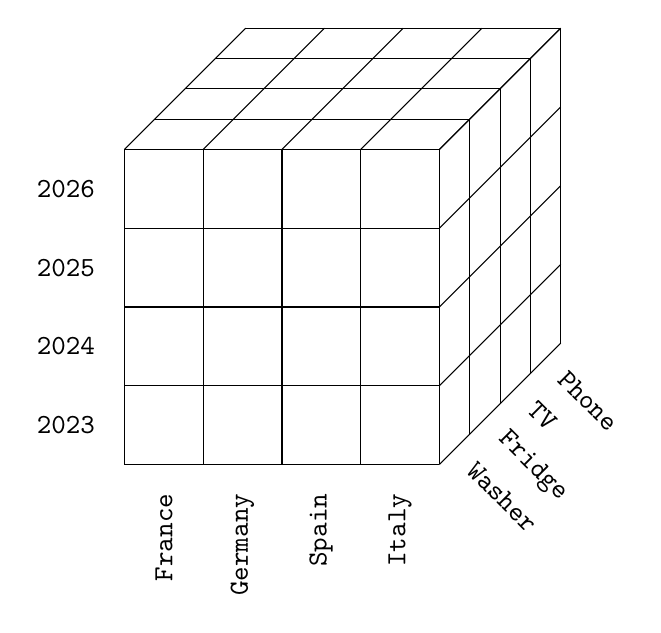
\begin{tikzpicture}[scale=1]
							% Cube of the initial data cube example
							\foreach \x in{0,...,4}
								{   \draw (0,\x ,4) -- (4,\x ,4);
									\draw (\x ,0,4) -- (\x ,4,4);
									\draw (4,\x ,4) -- (4,\x ,0);
									\draw (\x ,4,4) -- (\x ,4,0);
									\draw (4,0,\x ) -- (4,4,\x );
									\draw (0,4,\x ) -- (4,4,\x );
								}


							% Axis categories (highest granularity)
							% Time axis
							\node[anchor=east] at (-0.25,0.5,4) {\texttt{2023}};
							\node[anchor=east] at (-0.25,1.5,4) {\texttt{2024}};
							\node[anchor=east] at (-0.25,2.5,4) {\texttt{2025}};
							\node[anchor=east] at (-0.25,3.5,4) {\texttt{2026}};

							% Region axis 
							\node[anchor=east,rotate=90] at (0.5, -0.25, 4) {\texttt{France}};
							\node[anchor=east,rotate=90] at (1.5, -0.25, 4) {\texttt{Germany}};
							\node[anchor=east,rotate=90] at (2.5, -0.25, 4) {\texttt{Spain}};
							\node[anchor=east,rotate=90] at (3.5, -0.25, 4) {\texttt{Italy}};

							% Product axis
							\node[anchor=west,rotate=315] at (4.125, -0.125, 3.5) {\texttt{Washer}};
							\node[anchor=west,rotate=315] at (4.125, -0.125, 2.5) {\texttt{Fridge}};
							\node[anchor=west,rotate=315] at (4.125, -0.125, 1.5) {\texttt{TV}};
							\node[anchor=west,rotate=315] at (4.125, -0.125, 0.5) {\texttt{Phone}};

							% Node to fix the bounding box
							\node at (4, -1.5, 4) {};
						\end{tikzpicture}
					}
				};

				% Arrows between the two cubes
				\draw[->, very thick] ($(finer.east) + (0,0.25)$) -- ($(coarser.west) + (0,0.25)$);

				\node[text width=2.5cm, anchor=south] at (1.5,0.5) {
					\begin{block}{Roll Up}
						Switch to a coarser granularity.
					\end{block}
				};

				\draw[<-, very thick] ($(finer.east) + (0,-0.25)$) -- ($(coarser.west) + (0,-0.25)$);

				\node[text width=2.5cm, anchor=north] at (1.5,-0.5) {
					\begin{block}{Drill Down}
						Switch to a finer granularity.
					\end{block}
				};
			\end{tikzpicture}
		}
	\end{center}
\end{frame}


\begin{frame}{OLAP Operations: Pivot}
	\begin{center}
		\scalebox{0.875}{
			\begin{tikzpicture}[scale=1]

				% Start cube
				\node[anchor=east] at (0,0) (start) {
					\scalebox{0.8} {
						\begin{tikzpicture}[scale=1]
							% Cube of the initial data cube example
							\foreach \x in{0,...,4}
								{   \draw (0,\x ,4) -- (4,\x ,4);
									\draw (\x ,0,4) -- (\x ,4,4);
									\draw (4,\x ,4) -- (4,\x ,0);
									\draw (\x ,4,4) -- (\x ,4,0);
									\draw (4,0,\x ) -- (4,4,\x );
									\draw (0,4,\x ) -- (4,4,\x );
								}


							% Axis categories (highest granularity)
							% Time axis
							\node[anchor=east] at (-0.25,0.5,4) {\texttt{2023}};
							\node[anchor=east] at (-0.25,1.5,4) {\texttt{2024}};
							\node[anchor=east] at (-0.25,2.5,4) {\texttt{2025}};
							\node[anchor=east] at (-0.25,3.5,4) {\texttt{2026}};

							% Region axis 
							\node[anchor=east,rotate=90] at (0.5, -0.25, 4) {\texttt{France}};
							\node[anchor=east,rotate=90] at (1.5, -0.25, 4) {\texttt{Germany}};
							\node[anchor=east,rotate=90] at (2.5, -0.25, 4) {\texttt{Spain}};
							\node[anchor=east,rotate=90] at (3.5, -0.25, 4) {\texttt{Italy}};

							% Product axis
							\node[anchor=west,rotate=315] at (4.125, -0.125, 3.5) {\texttt{Washer}};
							\node[anchor=west,rotate=315] at (4.125, -0.125, 2.5) {\texttt{Fridge}};
							\node[anchor=west,rotate=315] at (4.125, -0.125, 1.5) {\texttt{TV}};
							\node[anchor=west,rotate=315] at (4.125, -0.125, 0.5) {\texttt{Phone}};

							% Node to fix the bounding box
							\node at (4, -1.5, 4) {};
						\end{tikzpicture}
					}
				};

				% Start cube with different orientation
				\node[anchor=west] at (3,0) (pivot) {
					\scalebox{0.8} {
						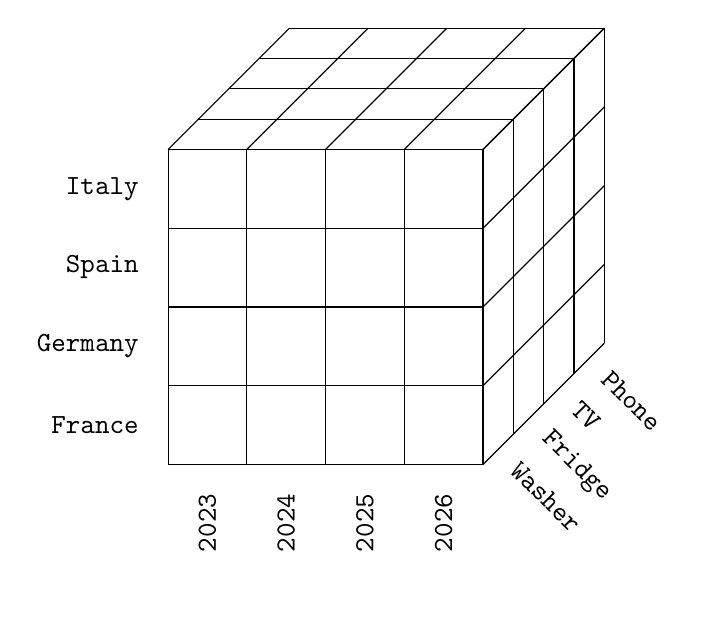
\begin{tikzpicture}[scale=1]
							% Cube of the initial data cube example
							\foreach \x in{0,...,4}
								{   \draw (0,\x ,4) -- (4,\x ,4);
									\draw (\x ,0,4) -- (\x ,4,4);
									\draw (4,\x ,4) -- (4,\x ,0);
									\draw (\x ,4,4) -- (\x ,4,0);
									\draw (4,0,\x ) -- (4,4,\x );
									\draw (0,4,\x ) -- (4,4,\x );
								}


							% Axis categories (highest granularity)
							% Region axis
							\node[anchor=east] at (-0.25,0.5,4) {\texttt{France}};
							\node[anchor=east] at (-0.25,1.5,4) {\texttt{Germany}};
							\node[anchor=east] at (-0.25,2.5,4) {\texttt{Spain}};
							\node[anchor=east] at (-0.25,3.5,4) {\texttt{Italy}};

							% Time axis 
							\node[anchor=east,rotate=90] at (0.5, -0.25, 4) {\texttt{2023}};
							\node[anchor=east,rotate=90] at (1.5, -0.25, 4) {\texttt{2024}};
							\node[anchor=east,rotate=90] at (2.5, -0.25, 4) {\texttt{2025}};
							\node[anchor=east,rotate=90] at (3.5, -0.25, 4) {\texttt{2026}};

							% Product axis
							\node[anchor=west,rotate=315] at (4.125, -0.125, 3.5) {\texttt{Washer}};
							\node[anchor=west,rotate=315] at (4.125, -0.125, 2.5) {\texttt{Fridge}};
							\node[anchor=west,rotate=315] at (4.125, -0.125, 1.5) {\texttt{TV}};
							\node[anchor=west,rotate=315] at (4.125, -0.125, 0.5) {\texttt{Phone}};

							% Node to fix the bounding box
							\node at (4, -1.5, 4) {};
						\end{tikzpicture}
					}
				};

				% Arrows between the two cubes
				\draw[->, very thick] ($(start.east) + (0,1.5)$) -- ($(pivot.west) + (0,1.5)$);
				\draw[<-, very thick] ($(start.east) + (0,1)$) -- ($(pivot.west) + (0,1)$);

				\node[text width=2.5cm, anchor=north] at (1.5,0.75) {
					\begin{block}{Pivot}
						Rotate the cube to provide a different view on the data.
					\end{block}
				};
			\end{tikzpicture}
		}
	\end{center}
\end{frame}
